{一元多项式相加的运算规则:{\textbf{对于两个一元多项式中所有指数相同的项,对应系数相加,若其和不为零,则构成``和多项式''中的一项;对于两个一元多项式中所有指数不相同的项,则分别复抄到``和多项式''中去。}}\\
用链式存储结构,实现一元多项式的相加。示意图如下:}

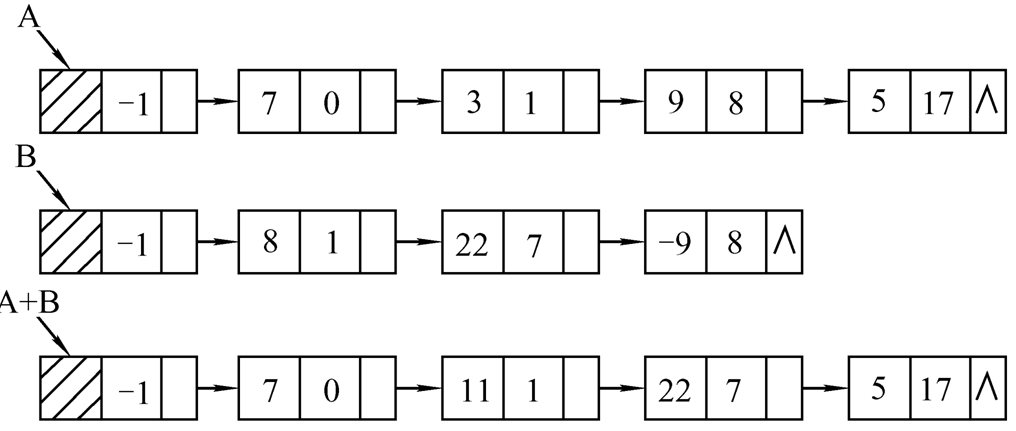
\includegraphics[width=3.22917in,height=1.37500in]{png-jpeg-pics/395B62F57E36F93B9A676676A26C7BD5.png}

{方法跟有序链表的合并有类似之处,首先对于结点的第二值域(指数),每个链表都是有序链表。如果两个一元多项式没有指数相同的项,则跟有序链表的合并是一模一样的。\\
{不同的是这里可能会有指数相同的项,多了一个相加第一值域的操作。若和不为零,则构成新的一个结点。若和为零,则两个结点``同归于尽''。}\\
考生根据这个思路和之前给的有序链表合并的代码,不难写出一元多项式的代码,由于不是重点部分,想看代码的考生请看严版教材。}
